% Paquets généraux
\documentclass[a4paper,12pt,titlepage,twoside]{article}
\usepackage[T1]{fontenc}
\usepackage[utf8]{inputenc}
\usepackage[french]{babel}
\addto\captionsfrench{%
  \renewcommand{\tablename}{Tableau}%
}
\usepackage[gen]{eurosym}
%\usepackage[dvips]{graphicx}
\usepackage{fancyhdr}
\usepackage{pdfpages} 
\usepackage{multido}
\usepackage{hyperref}
%\usepackage{textcomp}
\usepackage{schemabloc}
\usepackage[bitstream-charter]{mathdesign}
\usepackage{array}
\newcolumntype{P}[1]{>{\centering\arraybackslash}p{#1}}

\newcommand{\id}{54}
\newcommand{\nom}{Liaisons mécaniques}
\newcommand{\sequence}{04}
\newcommand{\num}{01}
\newcommand{\type}{TP}
\newcommand{\descrip}{Modélisation d'un solide. Comportement des liaisons mécaniques. Modéliser les mécanismes du laboratoire par un schéma cinématique, paramétré.}
\newcommand{\competences}{A3-C4: Analyse d'architecture et de comportement \\ &  Mod1-C1: Isolement d'un solide ou d'un système de solides \\ &  Mod2-C10-1: Modèle de solide indéformable \\ &  Mod2-C11: Modélisation géométrique et cinématique des mouvements entre solides indéformables \\ &  Mod2-C12: Modélisation cinématique des liaisons entre solides \\ &  Mod2-C15: Modélisation des actions mécaniques \\ &  Rés-C6: Utilisation d'un solveur ou d'un logiciel multi physique \\ &  Com1-C1: Différents descripteurs introduits dans le programme \\ &  Com2-C4: Outils de communication}
\newcommand{\nbcomp}{9}
\newcommand{\systemes}{Plateforme Stewart}
\newcommand{\systemessansaccent}{Plateforme Stewart}
\newcommand{\ilot}{2}
\newcommand{\ilotstr}{02}
\newcommand{\dossierilot}{\detokenize{Ilot_02 Plateforme Stewart}}
\newcommand{\imageun}{Plateforme}

\newcommand{\urlsysteme}{\href{https://www.costadoat.fr/systeme/57}{Ressources système}}
\newcommand{\matlabsimscape}{\href{https://github.com/Costadoat/Sciences-Ingenieur/raw/master/Systemes/Plateforme Stewart/Plateforme_Stewart_Simscape.zip}{Modèle Simscape}}
\newcommand{\solidworks}{\href{https://github.com/Costadoat/Sciences-Ingenieur/raw/master/Systemes/Plateforme Stewart/Plateforme_Stewart_Solidworks.zip}{Modèle Solidworks}}
\newcommand{\edrawings}{\href{https://github.com/Costadoat/Sciences-Ingenieur/raw/master/Systemes/Plateforme Stewart/Plateforme_Stewart.EASM}{Modèle eDrawings}}
\newcommand{\test}{Stewart_param1}
\newcommand{\testi}{Stewart_param2}
\newcommand{\testii}{Stewart_param3}
\newcommand{\testiii}{Stewart_param4}
\newcommand{\testiiii}{Stewart_euler}

\newcommand{\institute}{Lycée Dorian}

\usepackage{fancyvrb}
\usepackage{color}
\usepackage{xcolor}
\usepackage{colortbl}
\usepackage{helvet}
\renewcommand{\familydefault}{\sfdefault}
\usepackage{amsfonts}
\usepackage{amsmath}
%\usepackage{xspace}
\usepackage{varioref}
\usepackage{tabularx}
%\usepackage{floatflt}
\usepackage{graphics}
\usepackage{wrapfig}
\usepackage{textcomp}
\usepackage{tikz}
\usepackage{wrapfig}
\usepackage{gensymb}
\usepackage[percent]{overpic}
\usepackage[european]{circuitikz}
\usetikzlibrary{babel}
\usepackage{ifthen}
\usepackage{cancel}
\usepackage{etoolbox}
\usepackage{multirow}
%\usepackage{boxedminipage}
\definecolor{gris25}{gray}{0.75}
\definecolor{bleu}{RGB}{18,33,98}
\definecolor{bleuf}{RGB}{42,94,171}
\definecolor{bleuc}{RGB}{231,239,247}
\definecolor{rougef}{RGB}{185,18,27}
\definecolor{rougec}{RGB}{255,188,204}%255,230,231
\definecolor{vertf}{RGB}{103,126,82}
\definecolor{vertc}{RGB}{220,255,191}
\definecolor{forestgreen}{rgb}{0.13,0.54,0.13}
\definecolor{blcr}{rgb}{0.59,0.69,0.84}
\definecolor{blfr}{rgb}{0.32,0.51,0.75}
\definecolor{orfr}{rgb}{0.90,0.42,0.15}
\definecolor{orcr}{rgb}{0.90,0.65,0.50}
\definecolor{orangef}{rgb}{0.659,0.269,0.072}
\definecolor{orange}{rgb}{0.58,0.35,0.063}
\definecolor{orangec}{rgb}{0.43,0.32,0.25}
\definecolor{rcorrect}{rgb}{0.6,0,0}
\definecolor{sequence}{rgb}{0.75,0.75,0.75}
\definecolor{competences}{rgb}{0.61,0.73,0.35}
\definecolor{grisf}{HTML}{222222}
\definecolor{grisc}{HTML}{636363}
\definecolor{normal}{HTML}{4087c4}
\definecolor{info}{HTML}{5bc0de}
\definecolor{success}{RGB}{92,184,92}
\definecolor{warning}{RGB}{240,173,78}
\definecolor{danger}{RGB}{217,83,79}
\hypersetup{                    % parametrage des hyperliens
    colorlinks=true,                % colorise les liens
    breaklinks=true,                % permet les retours à la ligne pour les liens trop longs
    urlcolor= blfr,                 % couleur des hyperliens
    linkcolor= orange,                % couleur des liens internes aux documents (index, figures, tableaux, equations,...)
    citecolor= forestgreen                % couleur des liens vers les references bibliographiques
    }

% Mise en page
\pagestyle{fancy}

\setlength{\hoffset}{-18pt}
\setlength{\oddsidemargin}{0pt} 	% Marge gauche sur pages impaire2s
\setlength{\evensidemargin}{0pt} 	% Marge gauche sur pages paires
\setlength{\marginparwidth}{00pt} 	% Largeur de note dans la marge
\setlength{\headwidth}{481pt} 	 	% Largeur de la zone de tête (17cm)
\setlength{\textwidth}{481pt} 	 	% Largeu\textbf{r de la zone de texte (17cm)
\setlength{\voffset}{-18pt} 		% Bon pour DOS
\setlength{\marginparsep}{7pt}	 	% Séparation de la marge
\setlength{\topmargin}{-30pt} 		% Pas de marge en haut
\setlength{\headheight}{55pt} 		% Haut de page
\setlength{\headsep}{20pt} 		% Entre le haut de page et le texte
\setlength{\footskip}{30pt} 		% Bas de\textbf{ page + séparation
\setlength{\textheight}{700pt} 		% Hauteur de l'icone zone de texte (25cm)
\setlength\fboxrule{1 pt}
\renewcommand{\baselinestretch}{1}
\setcounter{tocdepth}{1}
\newcommand{\cadre}[2]
{\fbox{
  \begin{minipage}{#1\linewidth}
   \begin{center}
    #2\\
   \end{center}
  \end{minipage}
 }
}

\newcommand{\repon}[1]
{
~\ \\
\begin{tabular}{|m{\linewidth}|}
 \hline
\multido{}{#1}{\\ \hline}
\end{tabular}
}

\newcounter{num_quest} \setcounter{num_quest}{0}
\newcounter{num_rep} \setcounter{num_rep}{0}
\newcounter{num_cor} \setcounter{num_cor}{0}

\newcommand{\question}[1]{\refstepcounter{num_quest}\par
~\ \\ \parbox[t][][t]{0.15\linewidth}{\textbf{Question \arabic{num_quest}}}\parbox[t][][t]{0.85\linewidth}{#1}\par
}


\newcommand{\reponse}[3]
{\refstepcounter{num_rep}
\noindent
\rule{\linewidth}{.5pt}\\
\textbf{Question \arabic{num_rep}:} ~\ \\
\ifdef{\public}{\multido{\i=1+1}{#1}{~\ \\}#2}{#3}
}

\newcommand{\cor}
{\refstepcounter{num_cor}
\noindent
\rule{\linewidth}{.5pt}
\textbf{Question \arabic{num_cor}:} \\
}

\newcommand{\repcarre}[2]
{
~\ \\
\begin{tikzpicture}
\draw [fill=white] (0,0) rectangle +(\linewidth,#1);
\node[align=left] at (1.1,#2-0.3) {\textbf{Question #1:}};
\end{tikzpicture}
}

\newcommand{\titre}[1]
{\begin{center}
\cadre{0.8}{\huge #1} 
\end{center}
}


% En tête et pied de page
\lhead{\nom}
\rhead{
\includegraphics[width=2cm]{../../img/logo}}
\lfoot{\auteurun,\ \auteurdeux}
\cfoot{Page \thepage}

\fancypagestyle{documentreponse}{%
  \fancyhf{}
  \fancyhead[LO]{Nom: ........................ Prénom: ........................}
  \fancyhead[LE]{\nom}
  \fancyhead[RE,RO]{
\includegraphics[width=2cm]{../../img/logo}}
  \lfoot{Document réponse}
  \cfoot{Page \thepage}
   }
  
\fancypagestyle{correction}{%
  \fancyhf{}
  \lhead{\colorbox{danger}{\begin{minipage}{0.65\paperwidth} \textcolor{white}{\textbf{Correction}} \end{minipage}} }
  \rhead{
\includegraphics[width=2cm]{../../img/logo}}
  \lfoot{Renaud Costadoat, Françoise Puig}
  \rfoot{\colorbox{danger}{\begin{minipage}{0.5\paperwidth} \begin{flushright}\textcolor{white}{\textbf{Correction}}\end{flushright} \end{minipage}} }}

\fancypagestyle{correctioninfo}{%
  \fancyhf{}
  \lhead{\colorbox{danger}{\begin{minipage}{0.65\paperwidth} \textcolor{white}{\textbf{Correction}} \end{minipage}} }
  \rhead{
\includegraphics[width=2cm]{../../img/logo}}
  \lfoot{Renaud Costadoat, Juliette Genzmer, Willie Robert}
  \rfoot{\colorbox{danger}{\begin{minipage}{0.6\paperwidth} \begin{flushright}\textcolor{white}{\textbf{Correction}}\end{flushright} \end{minipage}} }}

\renewcommand{\footrulewidth}{0.4pt}

\usepackage{eso-pic}
\newcommand{\BackgroundPic}{%
\put(0,0){%
\parbox[b][\paperheight]{\paperwidth}{%
\vfill
\begin{center}
\hspace{0.5cm}\vspace{0.5cm}

\includegraphics[width=\paperwidth,height=\paperheight,%
keepaspectratio]{../../img/fond3}%
\end{center}
\vfill
}}}

\newcommand{\BackgroundPicdeux}{%
\put(25,-30){%
\parbox[b][\paperheight]{\paperwidth}{%
\vfill
\begin{center}
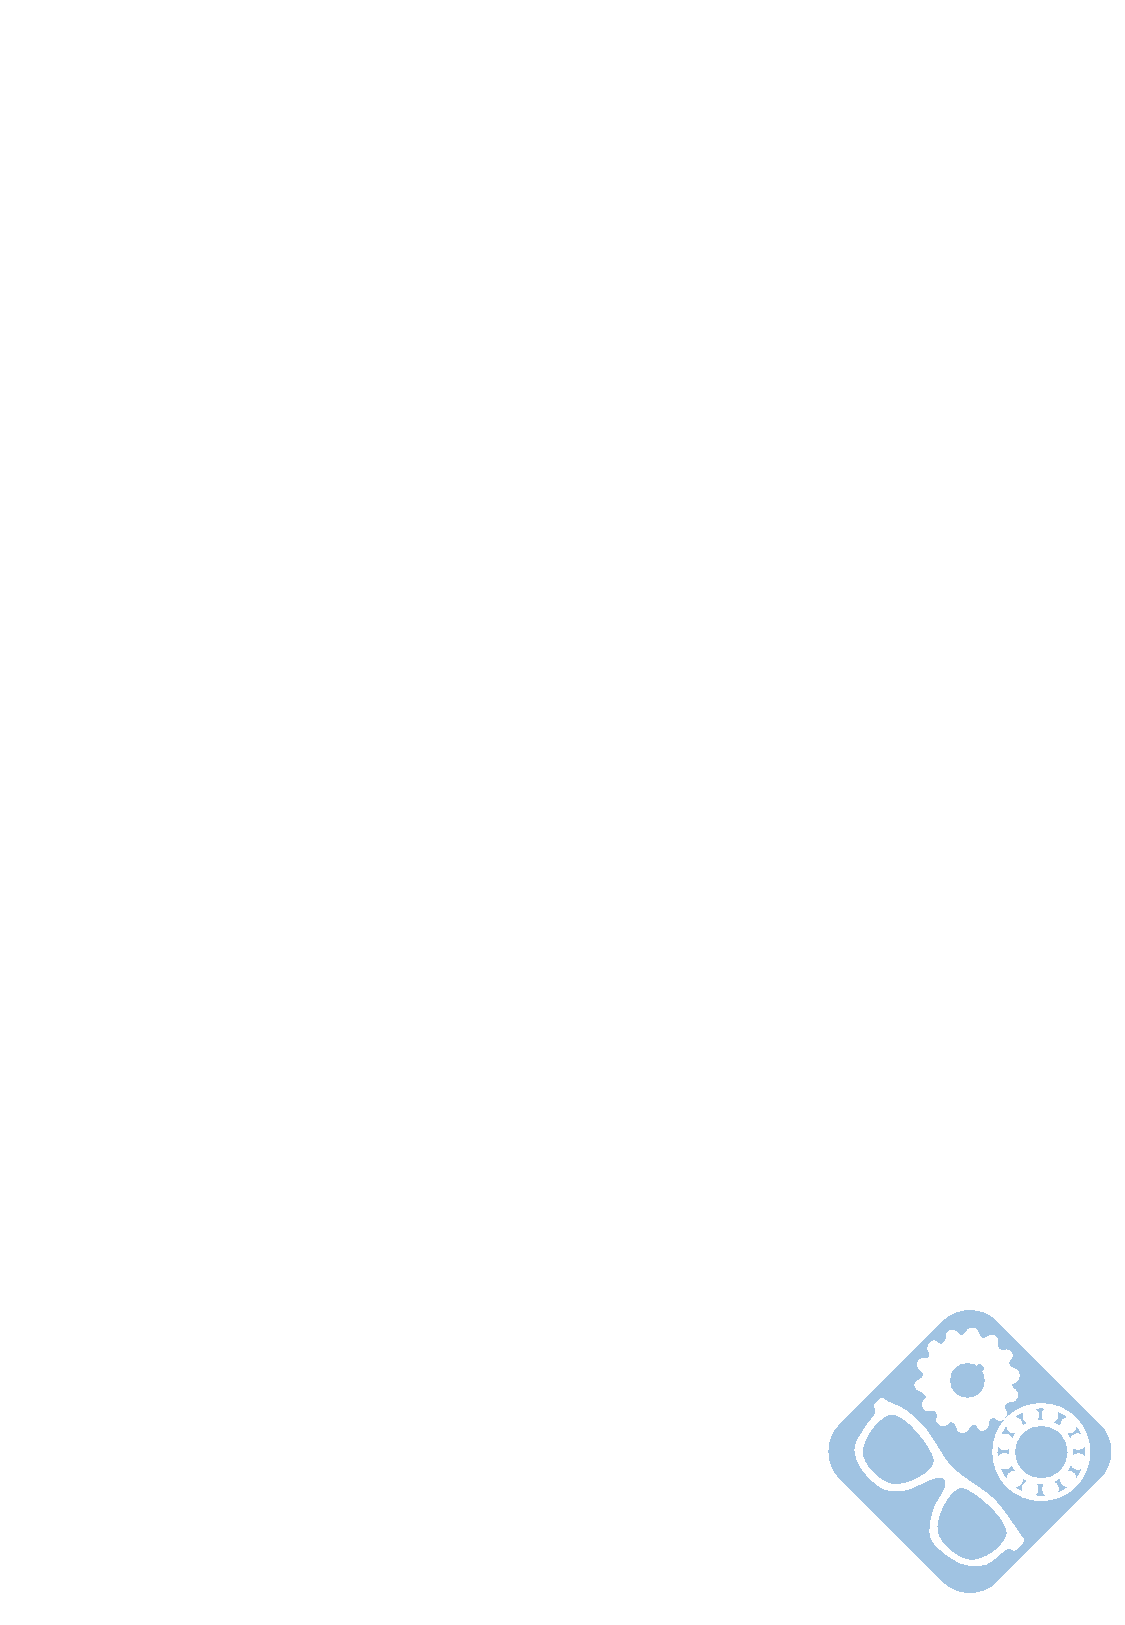
\includegraphics[width=\paperwidth,height=\paperheight,%
keepaspectratio]{../../img/fond4}%
\end{center}
\vfill
}}}

\begin{document}

\pagestyle{empty}

\AddToShipoutPicture*{\BackgroundPic}


\includegraphics[width=2cm]{../../img/logo}

\Huge{DS \num\ - \sujet}

\vspace{1cm}

\ifdef{\prive}{\begin{center}\colorbox{danger}{\Huge{Avec Correction}}\end{center}}{}

\begin{center}
\centering\huge{PTSI}
\end{center}

\vspace{2cm}


\begin{center}
\centering\Large{\jour}
\end{center}

\vspace{2cm}

\normalsize

\tableofcontents

\newpage

\AddToShipoutPicture{\BackgroundPicdeux}

\pagestyle{fancy}

\begin{center}
\Huge \sujet
\end{center}


\normalsize

\section{Présentation}

\subsection{Présentation de la laveuse}

\begin{figure}[!h]
\begin{minipage}{0.55\linewidth}
La société Nilfisk propose une large gamme d’engins de nettoyage des sols. Celle des laveuses autoportées répond aux besoins de lavage pour des surfaces de plusieurs milliers de km carrés. C’est par exemple le cas des sols de super et hyper-marché. Les qualités de ces machines résident dans leur sécurité d’usage, leur faible nuisance sur l’environnement, leur autonomie et leur maniabilité. Cette maniabilité impose des encombrements minimisés en largeur et des rayons de giration
très faibles.
\end{minipage} \hfill
\begin{minipage}{0.4\linewidth}
\centering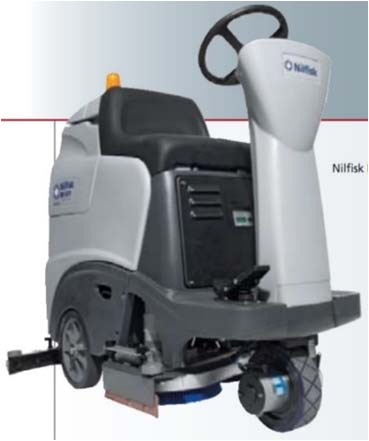
\includegraphics[width=0.8\linewidth]{img/img01}
 \caption{Laveuse autoportée}
 \label{img01}
 \end{minipage}
\end{figure}

\begin{figure}[!h]
\begin{minipage}{0.4\linewidth}
\centering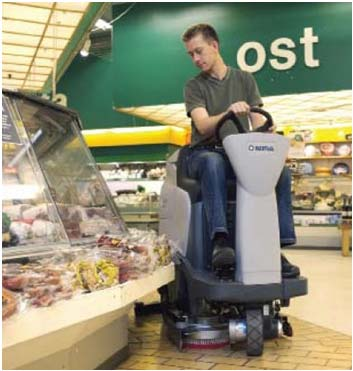
\includegraphics[width=0.8\linewidth]{img/img02}
 \caption{Technicien sur une laveuse autoportée}
 \label{img02}
\end{minipage} \hfill
\begin{minipage}{0.55\linewidth}
Le modèle étudié dans ce sujet est la laveuse BR 752 dont la structure du châssis à trois roues est privilégiée pour autoriser des rayons de giration très petits. Sur la gamme actuelle, la motorisation est assurée par la roue avant avec une machine à courant continu. Une évolution est envisagée qui conduirait à remplacer la motorisation avant par deux moteurs à l’arrière non orientables mais commandés en vitesse. Cette modification doit a minima maintenir les performances de la solution existante.
\end{minipage}
\end{figure}

Ce sujet a pour but d’analyser les différentes performances de la nouvelle laveuse.

\newpage

\subsection{Diagrammes fonctionnels}

\begin{figure}[!h]
\centering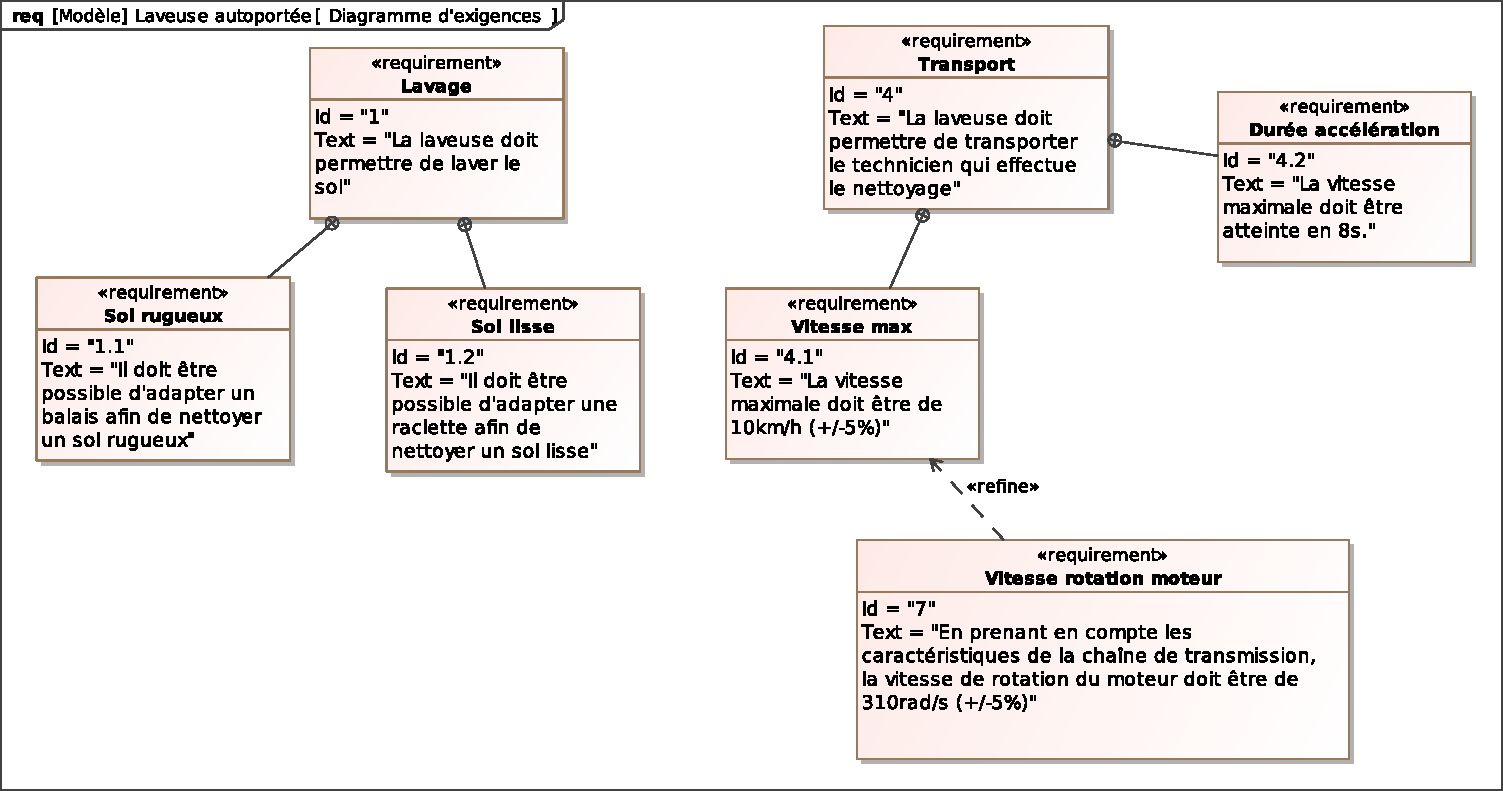
\includegraphics[width=0.8\linewidth]{img/Diagramme_d'exigences}
 \caption{Diagramme d'exigences du système}
 \label{img03}
\end{figure}

\begin{figure}[!h]
\centering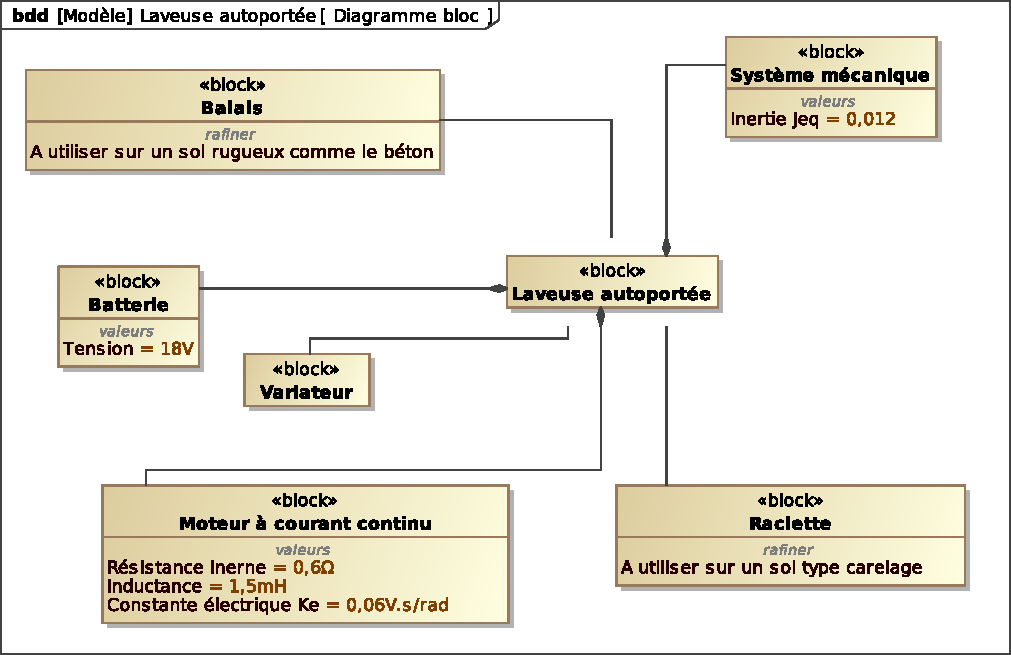
\includegraphics[width=0.8\linewidth]{img/Diagramme_bloc}
 \caption{Diagramme bloc du système}
 \label{img04}
\end{figure}

\question{Sur le diagramme bloc de la figure \ref{img04}, les losanges au bout des blocs \og Balais \fg, \og Raclette \fg et \og Variateur \fg ont été effacés. Donner pour chacun sa couleur et donner le nom de l'association qui correspond.}

\question{Compléter la chaîne d'énergie du document réponse en mettant le nom de la fonction dans le bloc et l'élément du système qui répond à cette fonction sur les pointillés.}

\section{Pilotage des moteurs}

Pour répondre à l'exigence \og Id=4 \fg, il a été décidé de ne pas asservir en vitesse les moteurs. Mais d'envoyer le profil de tension de la figure \ref{img05} lorsque le technicien appuie sur la pédale d'accélération.

\begin{figure}[!h]
\centering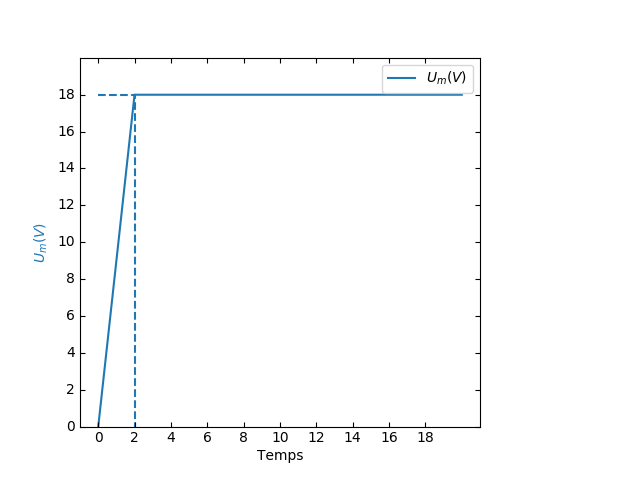
\includegraphics[width=0.6\linewidth]{img/tension}
 \caption{Tension d'alimentation du système}
 \label{img05}
\end{figure}

\question{Justifier qu'il est techniquement possible d'atteindre ce profil de tension à partir des caractéristiques des composants du système.}

~\

Dans un premier temps, il est nécessaire d'étudier le moteur à courant continu utilisé sur ce système.

\question{Donner les 4 équations qui régissent le comportement du moteur à courant continu (on négligera les frottements pour cette question). Doivent apparaître dans ces équations: $u_m(t)$, $\omega_m(t)$, $c_m(t)$, $i(t)$, $e(t)$, $K_e$, $K_t$, $R$, $J_{eq}$ et $L$.}

\question{Les conditions initiales sont nulles, écrire ces équations dans le domaine de Laplace, en citant le ou les théorèmes utilisés.}

\question{Écrire la fonction de transfert $H_m(p)=\frac{\Omega_m(p)}{U_m(p)}$ et la mettre sous la forme canonique.}

\question{Donner l'ordre, la classe et le gain de cette fonction de transfert.}

~\

On s'appuiera sur la forme canonique suivante pour la suite:
$H_m(p)=\frac{K}{1+\frac{2.\xi}{\omega_0}.p+\frac{p^2}{\omega_0^2}}$.

\question{Déterminer les formes littérales de $K$, $\xi$ et de $\omega_0$. Faire l'application numérique.}

\question{Montrer que l'on peut écrire cette fonction de transfert sous la forme \\ $H_m(p)=\frac{K}{(1+\tau_1.p)(1+\tau_2.p)}$.}

\question{Déterminer les valeurs numériques de $\tau_1$ et $\tau_2$. (Il est conseillé d'effectuer tous les calculs en numérique le plus rapidement possible (notamment $\Delta$)). Pour cela, on donne $\sqrt{3,98}=1,995$.}

\question{Montrer que l'on peut alors mettre la fonction de transfert sous la forme suivante $H_m(p)=\frac{K}{1+\tau_m.p}$ et déterminer $\tau_m$.}

~\

Dans la suite, nous allons considérer la partie du profil de tension telle que $t\in[0,2s]$.

\question{Déterminer la pente de la tension entre 0 et 2s. Mettre alors cette tension sous la forme $u_m(t)=\alpha.t$. Quelle est l'unité de $\alpha$ ?}

\question{Écrire $\Omega_m(p)$ la sortie de la fonction de transfert $H_m(p)$ lorsque l'entrée est $U_m(p)$.}

\question{En déduire $\omega_m(t)$ la sortie dans le domaine temporel lorsque l'entrée est $u_m(t)$.}

\question{Trouver la valeur de $\omega_m(t)$ pour $t=2s$. On donne $e^{-1}=0.37$.}

\section{Identification d'une réponse temporelle}

On donne la réponse suivante $s(t)$ pour un échelon unitaire $e(t)=1$.

\begin{figure}[!ht]
\centering
\includegraphics[width=0.8\linewidth]{img/fig01}
\caption{Tracé de la réponse temporelle s(t)}
\label{fig01}
\end{figure}

\question{Déterminer le $K$  de la fonction de transfert correspondante.}

\question{Déterminer le $\xi$ (à 0,1 près) de la fonction de transfert correspondante. On donne $\left(\frac{ln(2)}{\pi}\right)^2=0,05$.}

\question{Déterminer le $\omega_0$ de la fonction de transfert correspondante.}

\newpage

\cleardoublepage

%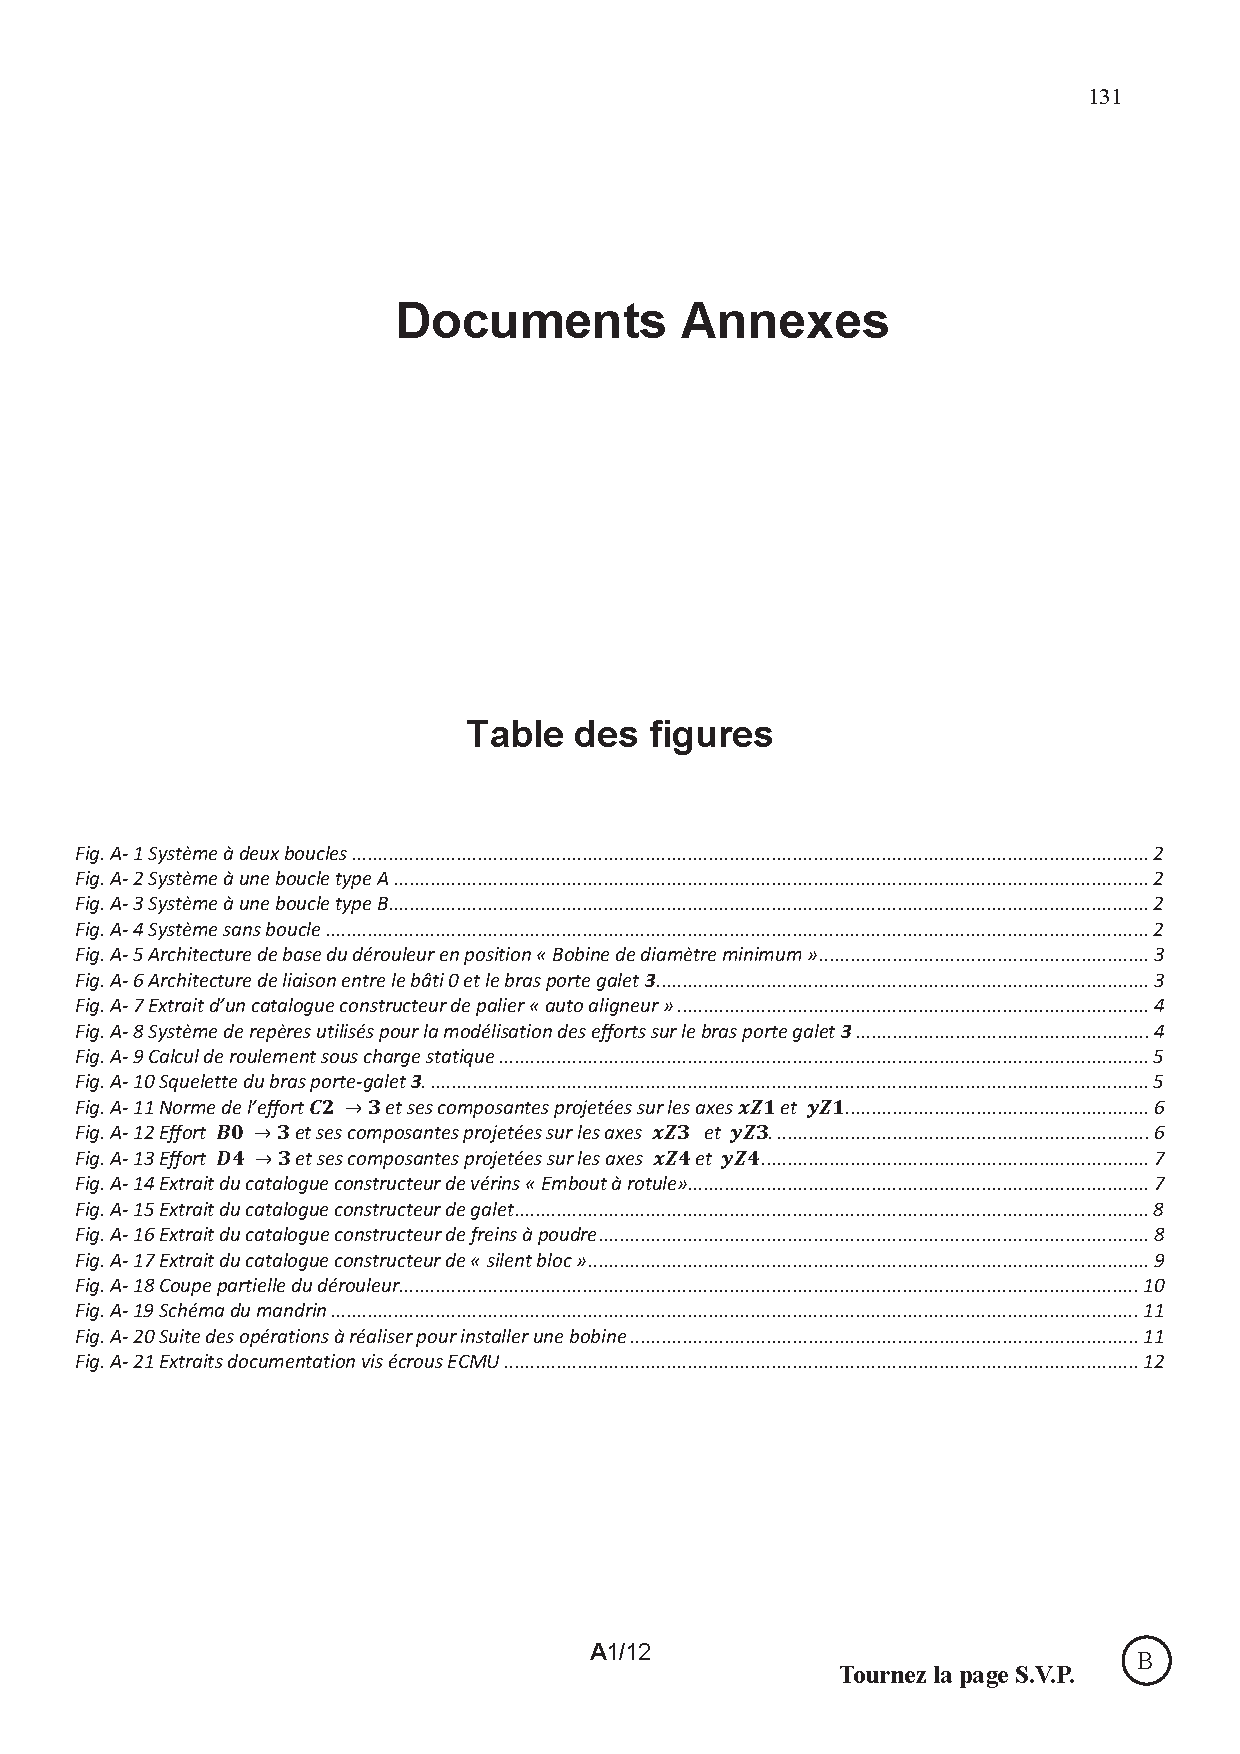
\includepdf[offset=5mm -10mm 0mm 0mm,pages=1]{img/annexes.pdf}

\newpage
\cleardoublepage

\pagestyle{documentreponse}

\section{Documents réponse}

\reponse{6}{}{Pour le \og Balais \fg et la \og Raclette \fg le losange est blanc (agrégation) car ces éléments ne sont pas obligatoires (leur installation dépend du contexte).

Pour le \og Variateur \fg il est noir (composition) car sans le variateur le système ne fonctionne pas.}

\reponse{0}{\begin{center}
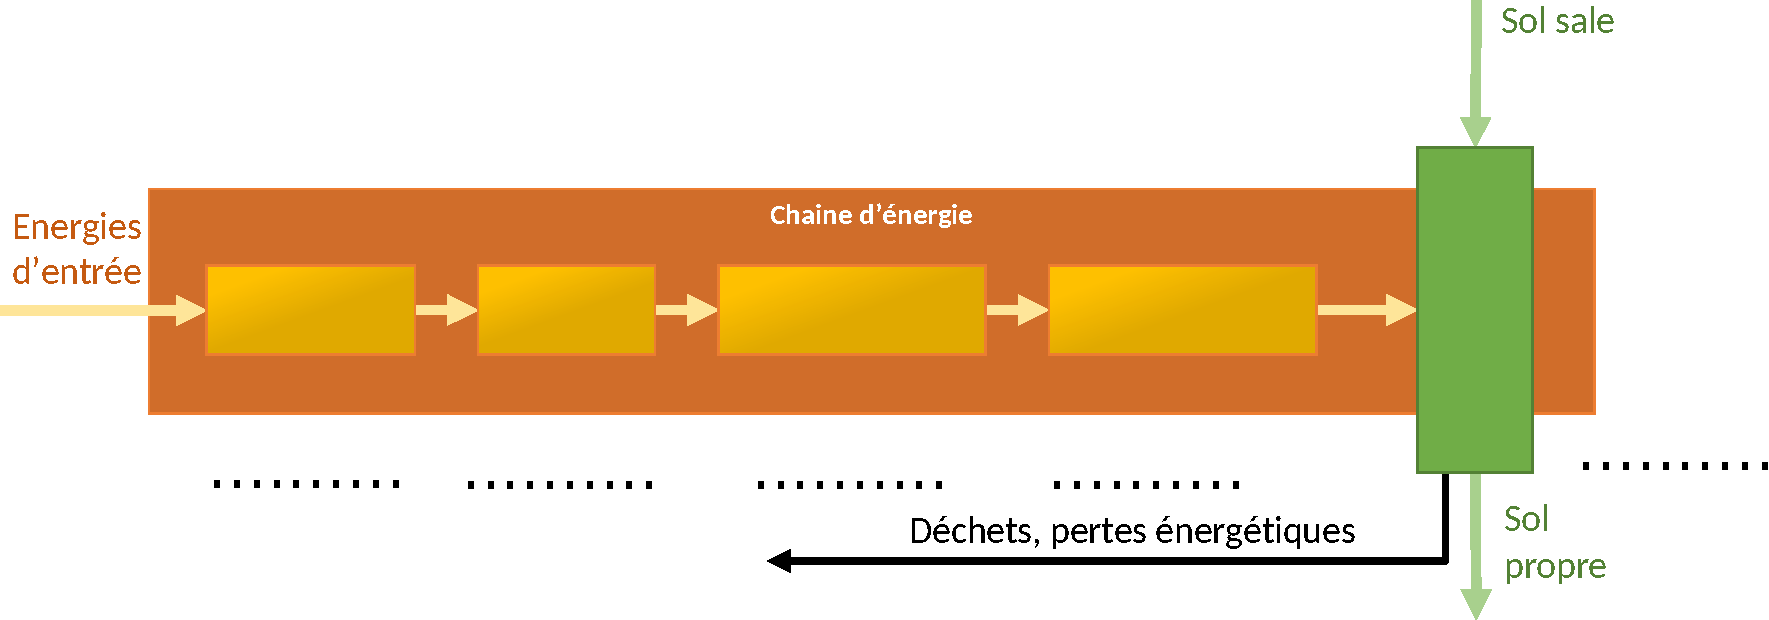
\includegraphics[width=0.8\linewidth]{img/Chaine_energie_vide.pdf}
\end{center}}{\begin{center}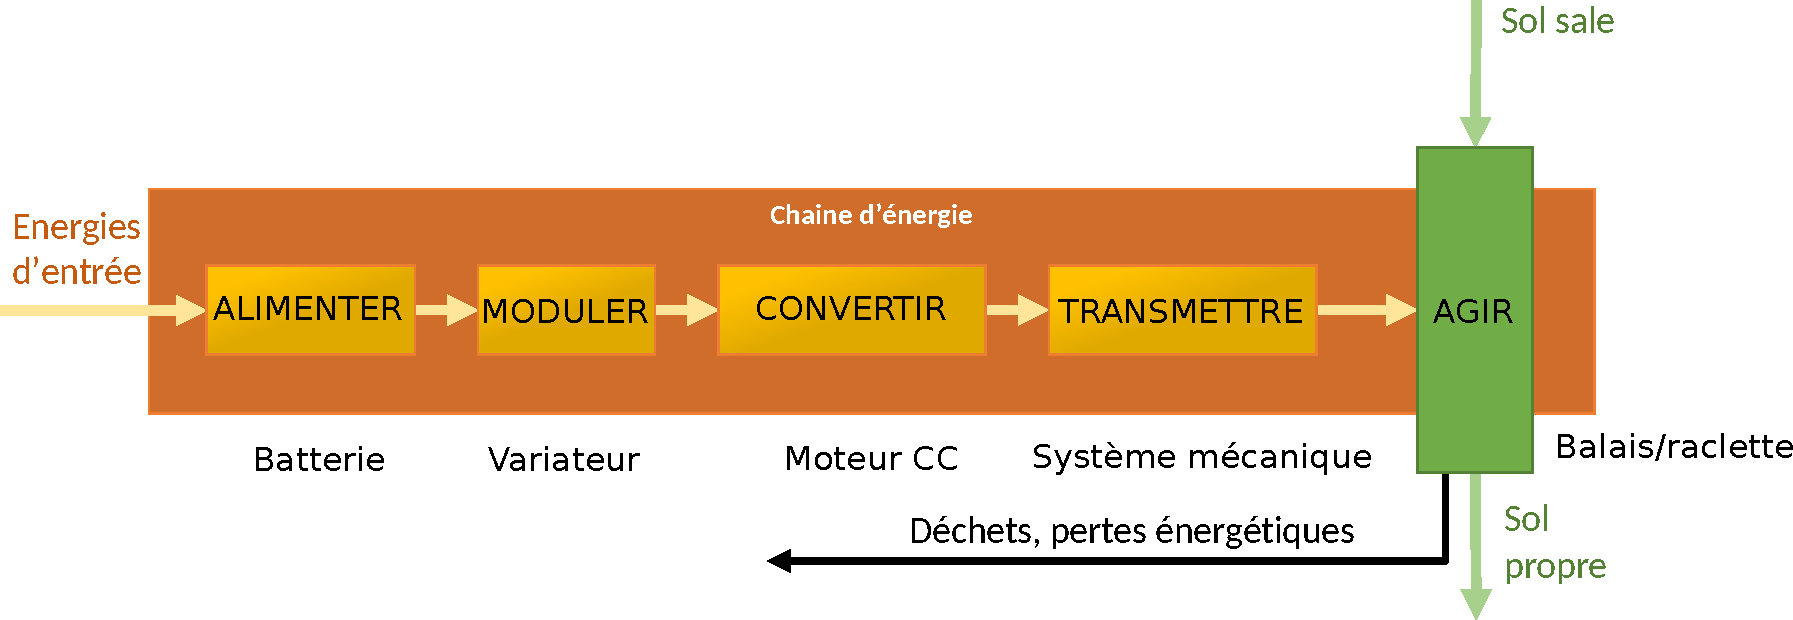
\includegraphics[width=0.8\linewidth]{img/Chaine_energie.pdf}\end{center}}

\reponse{7}{}{La tension maximale est de 18V, ce qui correspond à la tension de la batterie, ainsi, il est tout à fait possible de demander au variateur de fournir ce profil de tension.
}

\reponse{8}{}{
$u_m(t)=R.i(t)+L.\frac{di(t)}{dt}+e(t)$

$\omega_m(t)=K_e.e(t)$

$c_m(t)=K_t.i(t)$

$c_m(t)=J_{eq}.\frac{d\omega_m(t)}{dt}$
}

\newpage

\reponse{9}{}{
$U_m(t)=R.I(p)+L.p.I(p)+E(p)$

$\Omega_m(p)=K_e.E(p)$

$C_m(t)=K_t.I(p)$

$C_m(t)=J_{eq}.p.\Omega_m(p)$
}

\reponse{9}{}{
$H_m(p)=\frac{\frac{1}{K_e}}{1+\frac{R.J_{eq}}{K_e.K_t}.p+\frac{L.J_{eq}}{K_e.K_t}.p^2}$}

\reponse{5}{}{
Fonction de transfert d'ordre 2, de classe 0 et de gain $\frac{1}{K_e}$.
}

\reponse{12}{}{
$K=\frac{1}{0.06}=\frac{100}{6}\approx 16$

$\omega_0=\sqrt{\frac{K_e.K_t}{L.J_{eq}}}=\sqrt{\frac{0,06^2}{1,5.10^{-3}.0,012}}=\sqrt{\frac{6.6.10^{-4}}{1,5.12.10^{-6}}}=\sqrt{200}\approx14rad.s^{-1}$

$\xi=\frac{1}{2}.\frac{R.J_{eq}}{K_e.K_t}.\sqrt{\frac{K_e.K_t}{L.J_{eq}}}=
\frac{0,6.0,012.\sqrt{200}}{2.6.6.10^{-4}}=
\frac{6.12.10^{-4}.\sqrt{200}}{2.6.6.10^{-4}}=\sqrt{200}\approx14$
}

\newpage

\reponse{8}{}{
$\xi$ est plus grand que 1 (le discriminant du dénominateur est positif) donc les pôles de la fonction de transfert sont réels négatifs, donc il est possible de décomposer le polynôme du second ordre en un produit de deux polynômes du premier ordre.
}

\reponse{12}{}{
Pour trouver $\tau_1$ et $\tau_2$, on cherche $p_1$ et $p_2$.

$\Delta=\left(\frac{R.J}{K_e.K_t}\right)^2-4.\frac{L.J}{K_e.K_t}=\left(\frac{0,6.0,012}{0,06.0,06}\right)^2-4\frac{1,5.10^{-3}.0,012}{0,06.0,06}=\left(\frac{6.12.10^{-4}}{6.6.10^{-4}}\right)^2-\frac{6.12.10^{-6}}{6.6.10^{-4}}=2^2-0,02=3,98$

On a $b=\frac{R.J}{K_e.K_t}=2$ et $a=0,005$, donc
$p_1=\frac{-2-1,995}{0,01}=\frac{-3,995}{0,01}\approx{-400}$

$p_2=\frac{-2+1,995}{0,01}=\frac{-0,005}{0,01}\approx{-0.5}$

On a donc $\tau_1=\frac{1}{400}=0,0025$ et $\tau_2=2$.
}

\reponse{5}{}{
$\tau_1$ est négligeable devant $\tau_2$, donc on peut assimiler ce second ordre à un premier ordre avec $\tau_m=\tau_2=2$.
}

\reponse{3}{}{
$\alpha=9V.s^{-1}$
}

\reponse{4}{}{
$\Omega_m(p)=H_m(p).U_m(p)=\frac{K}{1+\tau_m.p}.\frac{\alpha}{p^2}$
}

\newpage

\reponse{10}{}{
$\Omega_m(p)=\frac{K}{1+\tau_m.p}.\frac{\alpha}{p^2}=\frac{A}{1+\tau_m.p}+\frac{B.p+C}{p^2}=\frac{A.p^2+B.p+C+B.\tau_m.p^2+C.\tau_m.p}{(1+\tau_m.p).p^2}$

Donc,

$C=K.\alpha$, $B+C.\tau_m=0$, donc $B=-\tau_m.K.\alpha$ et $A+B\tau_m=0$, donc $A=\tau_m^2.K.\alpha$.

Ainsi, $\Omega_m(p)=\frac{\tau_m^2.K.\alpha}{1+\tau_m.p}+\frac{-\tau_m.K.\alpha.p+K.\alpha}{p^2}$

Et donc, $\omega_m(t)=\tau_m.K.\alpha.e^{-\frac{t}{\tau_m}}+K.\alpha.t-\tau_m.K.\alpha$.

$\omega_m(t)=K.\alpha.\left(t-\tau_m.\left(1-e^{-\frac{t}{\tau_m}}\right)\right)$
}

\reponse{6}{}{
$\omega_m(2)=\frac{9}{0,06}.\left(2-2.\left(1-e^{-1}\right)\right)=150.(2-2.0,63)=150.(2-1,26)=150.(0,74)=74+37=111rad.s^{-1}$
}

\reponse{5}{}{
$K=\frac{s(+\infty)}{1}=2$
}


\reponse{6}{}{
D'après la figure, $0,5=e^{-\frac{\xi.\pi}{\sqrt{1-\xi^2}}}$, donc $-ln(2)=-\frac{\xi.\pi}{\sqrt{1-\xi^2}}$, donc $\xi^2=\frac{\left(\frac{ln(2)}{\pi}\right)^2}{1+\left(\frac{ln(2)}{\pi}\right)^2}$, donc $\xi\approx\sqrt{\frac{0,05}{1,05}}\approx\sqrt{\frac{1}{21}}\approx0,2$.}

\reponse{5}{}{
D'après la figure, $Tp\approx0,03$, or $\omega_0=\frac{2.\pi}{Tp.\sqrt{1-\xi^2}}$, donc $\omega_0\approx\frac{2.\pi}{Tp}\approx\frac{2.3}{0,03}\approx200rad.s^{-1}$.}

\end{document}

